\documentclass[pdfpagelabels=false, usepdftitle=false, aspectratio=169]{beamer}
\IfFileExists{beamerthemeUM.sty}{%
    \usetheme[navigation, sectiontitles]{UM}
}{%
    \usetheme{Madrid}
}

\usepackage{graphicx, lipsum}
\usepackage{xcolor} 
\usepackage[english]{babel}
\usepackage{natbib}
\usepackage{hyperref}
\graphicspath{{../}}

\hypersetup{
    colorlinks=true,
    linkcolor=cyan,
    filecolor=magenta,      
    urlcolor=cyan,
    pdftitle={Overleaf Example},
    pdfpagemode=FullScreen,
    }

% Set caption font size to \tiny (smallest size)
\setbeamerfont{caption}{size= \tiny}

% ----------------------
% title page information
% ----------------------

\title[CV-2025]{Computer Vision - 2026}
\subtitle{Week \#09. Face Recognition}

\author[A.Kornaev, K.Yakovlev]{
    Lectures by Alexei Kornaev \inst{1,2} \\
    Practical sessions by Kirill Yakovlev \inst{1,3}
}

\institute[UM]{
    \inst{1} The Center for Top-Level Educational Programs \\
    in AI, Innopolis University (IU), Innopolis \\
    \inst{2} RC for AI, National RC for Oncology \\
    n.a. N.N.Blokhin, Moscow \\
    \inst{3} Ak Bars Bank, Kazan
}

\date{\today}

\makeatletter
\@ifundefined{UMtitleframe}{%
    \newcommand{\UMtitleframe}{%
        \begin{frame}
            \titlepage
        \end{frame}
    }
}{}
\makeatother

% ---------------------
% begin of presentation
% ---------------------

\begin{document}
\UMtitleframe  % note that we *do not* use \titlepage

% ----Frame------------
\begin{frame}{Agenda}
    \tableofcontents
\end{frame}

% ----Frame------------
\section{Outcomes}
\begin{frame}{Outcomes}
    This week on \href{https://paperswithcode.com/task/face-recognition}{Face Recognition} aims to provide students with a comprehensive understanding of face detection and recognition techniques. By the end of this lecture, students will be able to:
    \begin{enumerate}
        \item Estimate the challenges in the domain, including pose variation, illumination changes, occlusion, ethics, and adversarial attacks.
        \item Understand and compare different face recognition architectures.
        \item Analyze loss functions like contrastive loss, triplet loss, and ArcFace loss for face recognition models.
        \item Implement face recognition systems using deep learning frameworks and estimate the results.
    \end{enumerate}
    \vfill
    \begin{description}
        \item[Key Takeaway:] Face recognition is a crucial technology in security, authentication, and social applications, but it also raises ethical concerns that must be addressed.
    \end{description}
\end{frame}

% ----Frame------------
\section{Challenges in FR}
\begin{frame}{Challenges in Face Recognition}
\scriptsize
\begin{block}{Overview of Challenges}
    Face recognition systems face several challenges that can significantly impact their performance. These include pose variation, illumination changes, occlusion, ethical concerns, and adversarial attacks.
\end{block}
\begin{itemize}
    \item \textbf{Pose Variation:} Faces can appear in different orientations, making it difficult to match them.
    \item \textbf{Illumination Changes:} Variations in lighting conditions can alter the appearance of faces.
    \item \textbf{Occlusion:} Parts of the face may be obscured by objects or other faces.
    \item \textbf{Ethics:} Privacy concerns and biases in face recognition systems.
    \item \textbf{Adversarial Attacks:} Deliberate attempts to fool face recognition systems.
\end{itemize}
% \begin{figure}
%     \centering
%     \includegraphics[width=0.45\textwidth]{figures/face_recognition_challenges.png}
%     \caption{\href{https://arxiv.org/abs/2004.02980}{Challenges in face recognition.}}
% \end{figure}
\end{frame}

% ----Frame------------
\begin{frame}{Pose Variation}
\scriptsize
\begin{block}{Pose Variation}
    Pose variation refers to the different orientations of a face relative to the camera. This can include frontal, profile, and oblique views.
\end{block}
\begin{itemize}
    \item \textbf{Impact:} Reduces the accuracy of face recognition systems.
    \item \textbf{Solutions:} Use of 3D models, multi-view training data, and pose-invariant features.
\end{itemize}
% \begin{figure}
%     \centering
%     \includegraphics[width=0.45\textwidth]{figures/pose_variation.png}
%     \caption{\href{https://arxiv.org/abs/2004.02980}{Pose variation in face recognition.}}
% \end{figure}
\end{frame}

% ----Frame------------
\begin{frame}{Illumination Changes}
\scriptsize
\begin{block}{\href{https://arxiv.org/abs/2004.02980}{Illumination Changes}}
    Illumination changes refer to variations in lighting conditions that can alter the appearance of a face.
\end{block}
\begin{itemize}
    \item \textbf{Impact:} Can cause significant changes in the appearance of facial features.
    \item \textbf{Solutions:} Normalization techniques, use of infrared imaging, and deep learning models trained under various lighting conditions.
\end{itemize}
% \begin{figure}
%     \centering
%     \includegraphics[width=0.45\textwidth]{figures/illumination_changes.png}
%     \caption{\href{https://arxiv.org/abs/2004.02980}{Illumination changes in face recognition.}}
% \end{figure}
\end{frame}

% ----Frame------------
\begin{frame}[fragile]{Occlusion}
\scriptsize
Occlusion occurs when parts of a face are obscured by objects (e.g., masks, sunglasses), other people, or environmental factors. It degrades recognition accuracy by hiding critical facial features.
\begin{minipage}[t]{0.2\textwidth} % Left column for the figure
    \vspace{45pt} % Align to the top
    \begin{figure}[h]
        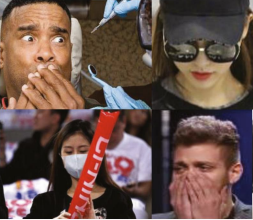
\includegraphics[width=\textwidth]{../figures/occlusion_examples.png}
        \caption{\href{https://ietresearch.onlinelibrary.wiley.com/doi/pdf/10.1049/bme2.12029}{Examples of occluded face images from the MAFA dataset \citep{zeng2021survey}.}}
    \end{figure}
\end{minipage}
\hfill
\begin{minipage}[t]{0.75\textwidth} % Right column for the content
    \vspace{0pt} % Align to the top
    \begin{block}{Understanding Occlusion}
        
    \end{block}
    \begin{itemize}
        \item \textbf{Impact:} 
        \begin{itemize}
            \item Loss of key features (e.g., eyes, mouth).
            \item State-of-the-art models like DeepFace or ArcFace suffer \textgreater30\% accuracy drop under heavy occlusion.
        \end{itemize}
        \item \textbf{Common Occlusions:} 
        % \begin{itemize}
            \textit{Masks} (e.g., medical masks).
            \textit{Accessories} (e.g., sunglasses, scarves).
            \textit{Environmental} (e.g., hands, hair).
        % \end{itemize}
        \item \textbf{Challenges:} 
        \begin{itemize}
            \item Partial face data limits recognition methods.
            \item Dynamic occlusions require real-time adaptation.
        \end{itemize}
    \end{itemize}
\end{minipage}
\end{frame}

% ----Frame------------
\begin{frame}{Solutions for Occlusion Handling}
\scriptsize
\begin{block}{Technical Approaches}
    Addressing occlusion requires robust feature extraction and reconstruction techniques.
\end{block}
\begin{itemize}
    \item \textbf{Partial Face Recognition:} 
    \begin{itemize}
        \item Train models on cropped facial regions (e.g., eyes-only, mouth-only). Use \textit{metric learning} to match partial and holistic embeddings.
    \end{itemize}
    \item \textbf{Attention Mechanisms:} 
    \begin{itemize}
        \item Focus on visible regions, e.g.\textit{Transformer Networks}) may prioritize non-occluded areas with attention \citep{liu2023patch}.
    \end{itemize}
    \item \textbf{Generative Models:} 
    \begin{itemize}
        \item Reconstruct occluded regions using GANs, Diffusion models.
    \end{itemize}
\end{itemize}
\begin{figure}
    \centering
    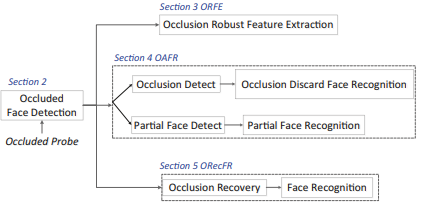
\includegraphics[width=0.23\textwidth]{../figures/FR_under_occlusion.png}
    \caption{\href{https://ietresearch.onlinelibrary.wiley.com/doi/pdf/10.1049/bme2.12029}{FR under occlusion \citep{zeng2021survey}.}}
\end{figure}
\end{frame}

% ----Frame------------
\begin{frame}[fragile]{Ethical Challenges in Face Recognition}
\scriptsize
\begin{block}{{Ethics: Privacy, Bias, and Misuse}}
    Face recognition systems raise critical ethical concerns, including privacy violations, algorithmic bias, and misuse in surveillance. These challenges undermine trust and fairness.
\end{block}
\begin{itemize}
    \item \textbf{Privacy Violations:} 
    \begin{itemize}
        \item \textit{Issue:} Unauthorized data collection and mass surveillance.
        % \item \textit{Example:} Use in authoritarian regimes to suppress dissent.
        \item \textit{Approach:} Implement strict data governance, anonymization, and user consent mechanisms.
    \end{itemize}
    \item \textbf{Algorithmic Bias:} 
    \begin{itemize}
        \item \textit{Issue:} Higher error rates for minorities, women, and darker-skinned individuals due to imbalanced training data.
        \item \textit{Example:} \href{https://doi.org/10.1145/3359246}{Buolamwini \& Gebru (2018)} showed 34\% error for dark-skinned women vs. 0.8\% for light-skinned men.
        \item \textit{Approach:} Curate diverse datasets, audit models for fairness, and adopt bias-mitigation techniques (e.g., reweighting losses).
    \end{itemize}
\end{itemize}
% \begin{figure}
%     \centering
%     \includegraphics[width=0.4\textwidth]{figures/ethics_bias.png}
%     \caption{\href{https://doi.org/10.1145/3359246}{Gender Shades study highlighting racial and gender bias.}}
% \end{figure}
\end{frame}

% ----Frame------------
\begin{frame}{Ethical Challenges: Solutions and Regulations}
\scriptsize
\begin{block}{{Regulatory Frameworks}}
    Addressing ethical issues requires technical, legal, and societal interventions.
\end{block}
\begin{itemize}
    \item \textbf{Technical Solutions:}
    \begin{itemize}
        \item \textit{Fairness-aware training:} Use fairness constraints during model optimization.
        \item \textit{Explainability:} Tools like LIME or SHAP to interpret model decisions.
    \end{itemize}
    \item \textbf{Legal Solutions:}
    \begin{itemize}
        \item \textit{Bans on mass surveillance:} EU's GDPR, proposed U.S. FR Act.
        \item \textit{Transparency laws:} Require disclosure of face recognition use cases.
    \end{itemize}
    \item \textbf{Societal Solutions:}
    \begin{itemize}
        \item Public awareness campaigns and ethical AI certification programs.
    \end{itemize}
\end{itemize}
% \begin{figure}
%     \centering
%     \includegraphics[width=0.35\textwidth]{figures/gdpr.png}
%     \caption{\href{https://gdpr-info.eu}{GDPR regulations for data privacy.}}
% \end{figure}
\end{frame}

% ----Frame------------
\begin{frame}[fragile]{Adversarial Attacks: Threat Models}
\scriptsize
\begin{block}{\href{https://arxiv.org/abs/1802.00420}{Adversarial Attacks in Face Recognition}}
    Adversarial attacks manipulate inputs to deceive face recognition systems. Common types include:
\end{block}
\begin{itemize}
    \item \textbf{Evasion Attacks:} 
    \begin{itemize}
        \item \textit{Goal:} Fool the system during inference (e.g., adversarial glasses).
        % \item \textit{Example:} \href{}{Eyeglass frames} causing misclassification.
    \end{itemize}
    \item \textbf{Poisoning Attacks:} 
    \begin{itemize}
        \item \textit{Goal:} Corrupt training data (e.g. injecting malicious samples).
    \end{itemize}
    \item \textbf{Model Inversion Attacks:} 
    \begin{itemize}
        \item \textit{Goal:} Reconstruct training data from model outputs (privacy breach).
    \end{itemize}
\end{itemize}
\begin{figure}
    \centering
    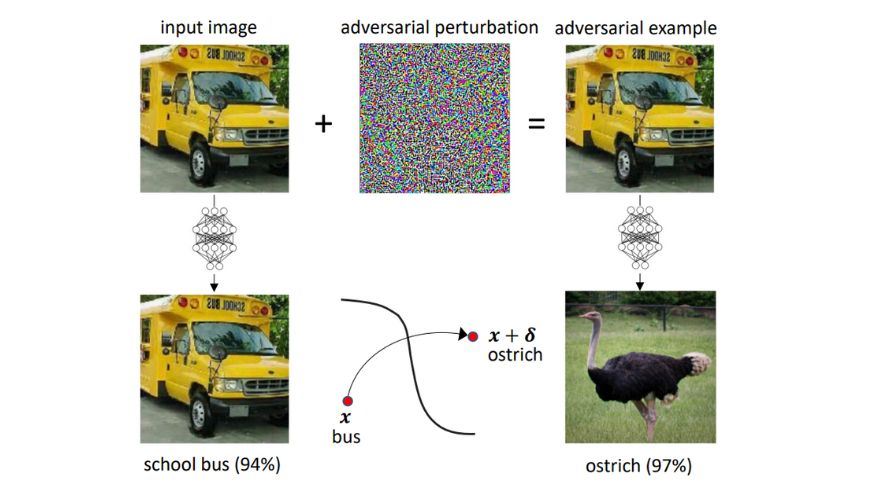
\includegraphics[width=0.34\textwidth]{../figures/adversarial_attack_example.jpg}
    \caption{{Adversarial noise attack.}}
\end{figure}
\end{frame}

% ----Frame------------
\begin{frame}{Defending Against Adversarial Attacks}
\scriptsize
\begin{block}{\href{https://arxiv.org/abs/1902.06705}{Robustness Strategies}}
    Mitigating adversarial attacks requires proactive defenses and robust model design.
\end{block}
\begin{itemize}
    \item \textbf{Adversarial Training:} 
    \begin{itemize}
        \item Train models on adversarial examples to improve robustness.
        \item \textit{Limitation:} Computationally expensive; does not generalize to all attacks.
    \end{itemize}
    \item \textbf{Input Preprocessing:} 
    \begin{itemize}
        \item Apply noise reduction, quantization, or JPEG compression to inputs.
    \end{itemize}
    \item \textbf{Detection Mechanisms:} 
    \begin{itemize}
        \item Deploy detectors to flag adversarial inputs (e.g., using inconsistency in feature space).
    \end{itemize}
    \item \textbf{Certified Defenses:} 
    \begin{itemize}
        \item Use mathematically proven robust models (e.g., randomized smoothing ).
    \end{itemize}
\end{itemize}
% \begin{figure}
%     \centering
%     \includegraphics[width=0.4\textwidth]{figures/adversarial_training.png}
%     \caption{\href{https://arxiv.org/abs/1706.06083}{Adversarial training process.}}
% \end{figure}
\end{frame}

% ----Frame------------
\section{{Traditional FR Methods}}
\begin{frame}[fragile]{Traditional Face Recognition Methods}
\scriptsize
Early approaches relied on dimensionality reduction and handcrafted features.
\begin{minipage}[t]{0.25\textwidth} % Left column for the figure
    \vspace{50pt} % Align to the top
    \begin{figure}[h]
        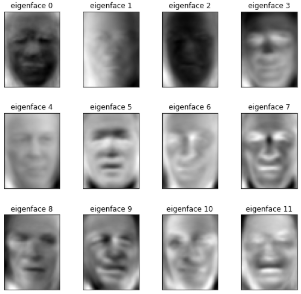
\includegraphics[width=\textwidth]{../figures/eigenfaces.png}
        \caption{\href{https://doi.org/10.1145/114191.114242}{Eigenfaces \citep{turk1991eigenfaces}.}}
    \end{figure}
\end{minipage}
\hfill
\begin{minipage}[t]{0.70\textwidth} % Right column for the content
    \vspace{0pt} % Align to the top
    \begin{block}{\href{https://doi.org/10.1145/114191.114242}{Linear Methods}}
        
    \end{block}
    \begin{itemize}
        \item \textbf{Eigenfaces \citep{turk1991eigenfaces}:} 
        \begin{itemize}
            \item Uses PCA to project faces into a low-dimensional subspace.
            \item Maximizes variance to capture dominant facial features.
        \end{itemize}
        \item \textbf{LBPH (Local Binary Patterns Histogram):} 
        \begin{itemize}
            \item Encodes texture patterns using local binary operators.
            \item Robust to monotonic illumination changes but struggles with pose/occlusion.
        \end{itemize}
    \end{itemize}
    % \textbf{Limitations:} 
    % \begin{itemize}
    %     \item Shallow representations fail to capture non-linear variations (e.g., expressions, aging).
    %     \item Manual feature engineering limits scalability.
    % \end{itemize}
\end{minipage}
\end{frame}

% ----Frame------------
\section{Deep Learning for FR}
\begin{frame}[fragile]{Deep Learning Architectures for Face Recognition}
\scriptsize
 Deep learning models learn discriminative embeddings by optimizing metric-based losses.
\begin{minipage}[t]{0.2\textwidth} % Left column for the figure
    \vspace{50pt} % Align to the top
    \begin{figure}[h]
        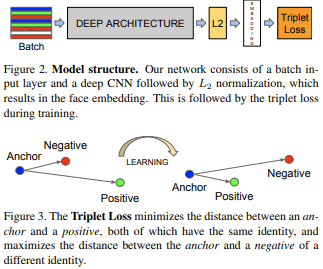
\includegraphics[width=\textwidth]{../figures/facenet_intuition.png}
        \caption{\href{https://arxiv.org/abs/1503.03832}{FaceNet embeddings \citep{schroff2015facenet, deng2019arcface}.}}
    \end{figure}
\end{minipage}
\hfill
\begin{minipage}[t]{0.75\textwidth} % Right column for the content
    \vspace{0pt} % Align to the top
    \begin{block}{\href{https://arxiv.org/abs/1503.03832}{Key Architectures}}
       
    \end{block}
    \begin{itemize}
        \item \textbf{Siamese Networks \citep{koch2015siamese}:} 
        \begin{itemize}
            \item Twin nets with shared weights for similarity learning.
            \item \textit{Contrastive loss} minimizes distances% between same-class pairs and maximizes it for different classes.
        \end{itemize}
        \item \textbf{FaceNet \citep{schroff2015facenet}:} 
        \begin{itemize}
            \item Maps faces to a compact 128D Euclidean space.
            \item Uses \textit{triplet loss}: \(\mathcal{L} = \max(||f(a) - f(p)||^2 - ||f(a) - f(n)||^2 + \alpha, 0)\), where \(a\)=anchor, \(p\)=positive, \(n\)=negative.
        \end{itemize}
        \item \textbf{ArcFace \citep{deng2019arcface}:} 
        \begin{itemize}
            \item Adds an \textit{additive angular margin} \(m\) to the loss.
            \item Enforces compactness and separation.
        \end{itemize}
    \end{itemize}
\end{minipage}
\end{frame}

% ----Frame------------
\begin{frame}[fragile]{Loss Functions in Face Recognition}
\scriptsize
\begin{block}{\href{https://arxiv.org/abs/1901.05555}{Metric Learning Objective}}
    A loss enforces that embeddings of the same identity are closer than those of different identities.
\end{block}
\begin{itemize}
    \item \textbf{Contrastive Loss :} %%\citep{hadsell2006dimensionality}
    \[
    \mathcal{L} = \frac{1}{2N} \sum_{i=1}^N y_i \cdot d_i^2 + (1 - y_i) \cdot \max(\alpha - d_i, 0)^2
    \]
    where \(y_i = 1\) for same-class pairs, \(d_i\)=embedding distance, \(\alpha\)=margin.
    \item \textbf{Triplet Loss \citep{schroff2015facenet}:} 
    \[
    \mathcal{L} = \sum_{i=1}^N \max\left(||f(a_i) - f(p_i)||^2 - ||f(a_i) - f(n_i)||^2 + \alpha, 0\right)
    \]
    \item \textbf{ArcFace Loss \citep{deng2019arcface}:} 
    \[
    L = -\frac{1}{N} \sum_{i=1}^{N} \log \frac{e^{s \cos(\theta_{y_i} + m)}}{e^{s \cos(\theta_{y_i} + m)} + \sum_{j \neq y_i} e^{s \cos(\theta_j)}}
    \]
    where \(s\)=scaling factor, \(m\)=angular margin, \(\theta\)=angle between weight and feature.
    % \end{itemize}
\end{itemize}
\end{frame}

% ----Frame------------
\begin{frame}[fragile]{Evaluation Metrics}
\scriptsize
Metrics vary based on the task: verification (1:1) or identification (1:N).
\begin{minipage}[t]{0.3\textwidth} % Left column for the figure
    \vspace{50pt} % Align to the top
    \begin{figure}[h]
        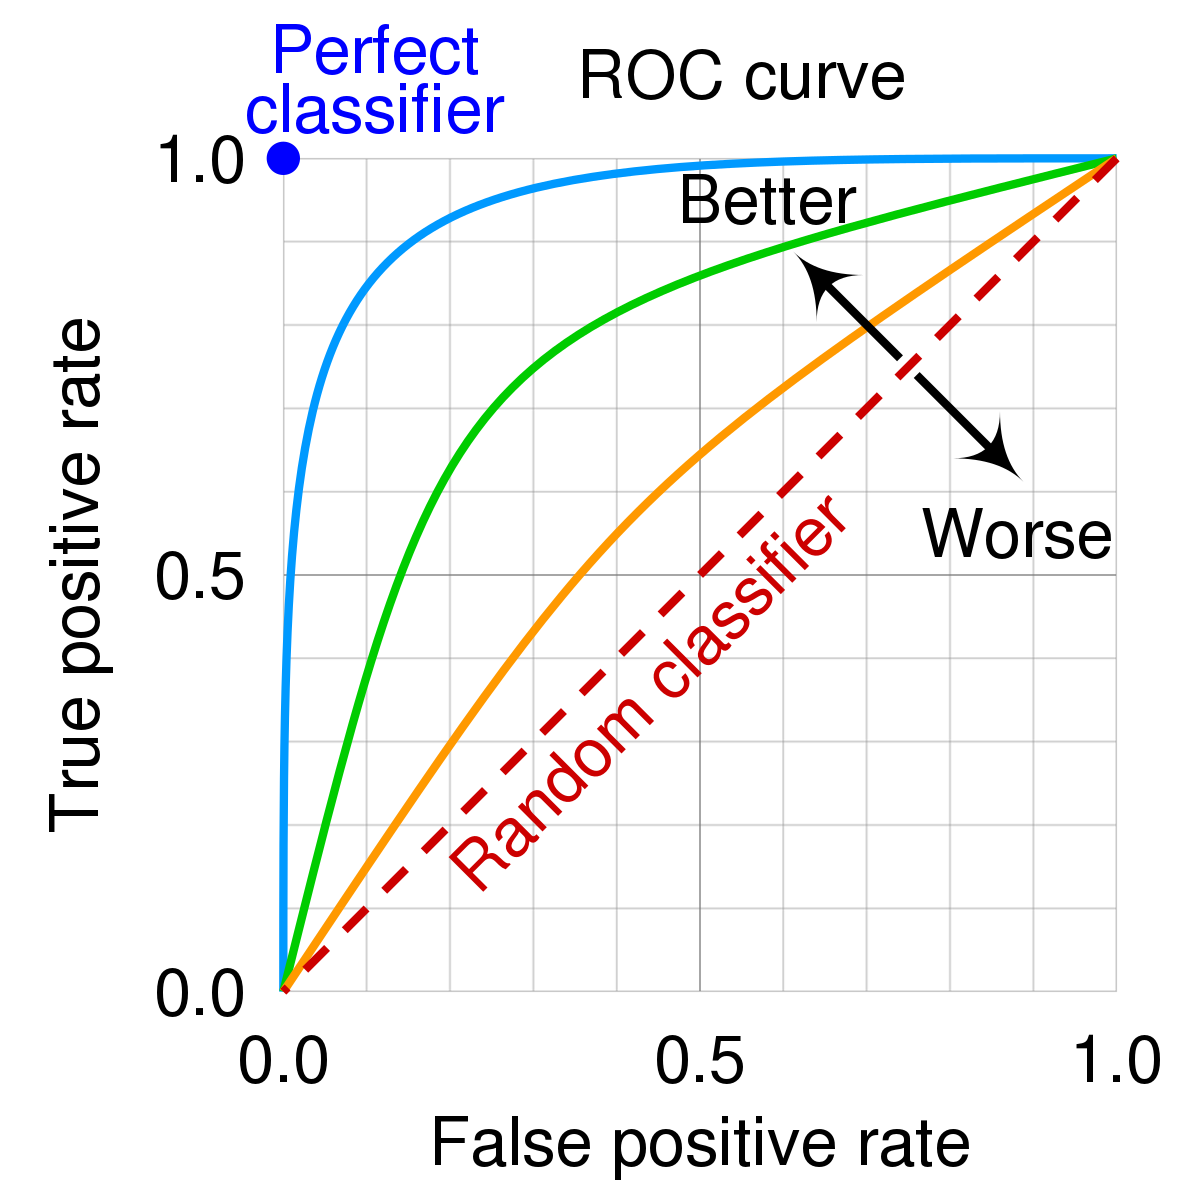
\includegraphics[width=\textwidth]{../figures/ROC.png}
        \caption{\href{https://vis-www.cs.umass.edu/lfw/}{ROC curve \citep{huang2008labeled}.}}
    \end{figure}
\end{minipage}
\hfill
\begin{minipage}[t]{0.65\textwidth} % Right column for the content
    \vspace{0pt} % Align to the top
    \begin{block}{\href{https://vis-www.cs.umass.edu/lfw/}{Performance Assessment}}
        
    \end{block}
    \begin{itemize}
        \item \textbf{Verification:} 
        \begin{itemize}
            \item \textit{False Acceptance Rate (FAR):} Incorrectly accepting impostors.
            \item \textit{False Rejection Rate (FRR):} Incorrectly rejecting genuine users.
            \item \textit{Equal Error Rate (EER):} FAR = FRR.
        \end{itemize}
        \item \textbf{Identification:} 
        \begin{itemize}
            \item Rank-1 accuracy: Top-1 match rate.
            \item Cumulative Match Curve (CMC).
        \end{itemize}
        \item \textbf{Benchmarks:} 
        \begin{itemize}
            \item LFW (Labeled Faces in the Wild): 99.8\% accuracy for ArcFace.
            \item MegaFace: Tests scalability (1M distractors).
        \end{itemize}
    \end{itemize}
    \textbf{Key Insight:} Trade-off between FAR and FRR defines security vs. usability.
\end{minipage}
\end{frame}


% ----Frame------------
\section{Conclusion \& Discussion}
\begin{frame}{Conclusion \& Discussion}
    \textbf{Strengths and Limitations}
    \begin{itemize}
        \item \textbf{Traditional Methods (PCA/LBP):} Interpretable but fail on complex variations
        \item \textbf{Deep Embeddings (FaceNet):} Robust features but need massive labeled data
        \item \textbf{ArcFace:} Superior separation but sensitive to alignment
    \end{itemize}

    \textbf{Future Directions}
    \begin{itemize}
        \item Vision Transformers for face recognition
        \item Federated learning for privacy-preserving biometrics
        \item Synthetic data generation with diffusion models
    \end{itemize}

    \textbf{Open Challenges}
    \begin{itemize}
        \item Ethical deployment: Bias mitigation \& fairness
        \item Robustness to adversarial attacks
        \item Cross-ethnicity generalization
    \end{itemize}

    % \begin{figure}
    %     \centering
    %     \includegraphics[width=0.4\textwidth]{figures/ethical_ai.png}
    %     \caption{Balancing accuracy with ethical considerations in face recognition.}
    % \end{figure}
\end{frame}

% ----Frame------------
\begin{frame}{Key Takeaways \& Practical Insights}
    \textbf{Student Summary}
    \begin{itemize}
        \item \textbf{Traditional Methods:} 
        \begin{itemize}
            \item Simple but limited (PCA/LBP struggle with pose/lighting)
            \item Foundation for understanding feature engineering
        \end{itemize}
        \item \textbf{Deep Learning:} 
        \begin{itemize}
            \item Embeddings + metric loss = Robustness
            \item Automatically learns hierarchical features
        \end{itemize}
    \end{itemize}

    \textbf{The Loss Function Revolution}
    \begin{itemize}
        \item \textcolor{blue}{Contrastive Loss:} Pair-based similarity learning
        \item \textcolor{blue}{Triplet Loss:} Relative distance optimization
        \item \textcolor{blue}{ArcFace:} Angular margin for better separation
    \end{itemize}

    % \textbf{Evaluation in Practice}
    % \begin{figure}
    %     \centering
    %     \includegraphics[width=0.8\textwidth]{figures/metrics_tradeoff.png}
    %     \caption{Security vs Usability trade-off: FAR vs FRR \citep{phillips2018face}}
    % \end{figure}
    
    % \begin{itemize}
    %     \item \textbf{Security Systems:} Low FAR (False Acceptance Rate)
    %     \item \textbf{Usability Focus:} Low FRR (False Rejection Rate) 
    % \end{itemize}
\end{frame}

% ----Ref Frame--------
\begin{frame}{Bibliography}
\tiny 
\bibliographystyle{plainnat}
% \bibliographystyle{plain}
\bibliography{../references}
\end{frame}

\end{document}

